\chapter{Background}\label{chap:background}
% This chapter will perform a breath-first explanation on the contents related
% with the thesis. The extension of the contents explained here can be seen as
% monotone function over the number of missing pages to attain the requirements.
%
% Some topics are indeed important as its the case of factor graphs.
% Others like:
%  - classification (SVM, multi-class, kernel-trick),
%  - features (SIFT, GIST),
%  - Basic Bayes theory and probabilistic review
% are included for fun of the reader in case it inquires himself how to deal
% with the low-levels features we propose using.
%
% ---
% PS: This is the chapter that will be used to fill with unnecessary crap
% in case they really annoy me with the number of pages. Every other chapter
% will strive to be really required and be a masterpiece.
%

One of the interesting facts about high-level problems is that they often require a
broad overview of the whole system and several concepts. For example in the case of
this thesis approach to novelty detection on semantic knowledge it becomes first
important to understand how classification of already known categories is performed.
I.e.\ understand how can
lower\hyp{}level classifiers be represented, how to obtain those representations from
training data, and how to use those them to infer new classifications from those models.
It is also important to know how to model several of those classifications with
probabilistic relations in a unified model and how to infer information on those.

This chapter tries to briefly introduce the reader to those aspects. The presented material
is not complete, it serves only to give directions and cues to the reader on how the several
subproblems of visual place classification can be solved. 
Where appropriate it refers to articles or textbooks that present the introduced techniques.

\section{Classification}
Classification deals with the problem of identifying classes or groups that lie underneath
the sensed data. It is expected that the presence of a underlying concept is involved on the
generation of the data that is sensed, and the system tries to infer that underlying concept
without directly observe it.

Often the sensed data is just to large to be directly handled within a classifier. In those
cases classifiers work on a small subset of features extracted from the data. Those features
should avoid discard important information and if correctly employed should turn the classification
easier.

\subsection{Recognition and Categorization}
Classification can target very different types of classes, as it is not clear on which classes
the system is interested in distinguish. For example the system maybe interested in distinguish
specific instances or interested in detecting a wide group of instances matching a
common category. E.g. distinguish a specific room: room 304 in the 3rd floor, from a generic room
category: a library.

Based on the type of desired learning system, the available features and the required generalization
specifications a wide range of machine-learning methods can be used. And no single method
is expected to handle all the problems with optimal performance.
The methods can go from statistical classification, neural networks, nearest neighbours,
decision trees, support vector machines to others like graphical models, clustering,
Gaussian mixture models, hidden Markov models, principal component analysis~\cite{bishop2006pattern}.

This background chapter does not aims at describing all the classification methods, but at
introducing the concept of classifier and to use them to extract information from low\hyp{}level
features. In that sense only \glspl{SVM} will be generally described, for more information
on others the reader is welcome to check the vast literature in pattern recognition and machine
learning such as the standard textbook cited above.

\subsection{Supervised and Unsupervised Training}
It is often impossible to manually specify the information needed to correctly classify samples.
There is also interest to make systems flexible and allow them to learn and adapt based solely
on the available data. In that sense the option is to train classifiers from available data.
The training methods are often separated as:

\begin{description}
\item[Supervised Methods] assume the existent of a supervisor that is able to give the
ground\hyp{}truth. With it the algorithm tries to learn the best description that matches
the given labelled data.
\item[Unsupervised Methods] try to learn classes without any extra information. The methods
have to figure out how many and which classes seem more reasonable to be modelled.
\end{description}

\subsection{Discriminative and Generative Models}
\label{sec:discriminative-vs-generative}
After constructing a classifier from the information available either in form of
available knowledge on the task in hand and from acquired data samples, the agent
ends up with a model that represents the knowledge it believes to be suitable to
solve the task.

The produced model differs a lot based on the type of classifier but they can be
distinguished in two different categories:
\begin{description}
\item[Discriminative models] are only able to classify samples in the known categories.
\item[Generative models] model the full probability relation between sensed
features and classes. With that it becomes possible to use the learned model to generate
new samples.
\end{description}


\subsection{Multi-Class Classification}
\label{sec:multiclass-classifiers}
Most classifiers methods are designed as two-class classifier and do not
natively support multi-class classification problems.
The most common approach is to try to approach multi-class problems by
by combining several two-class classifiers and perform a voting scheme or other
integrating method based on the confidence of the individual two-class classifiers.
For example:

\begin{description}
\item[One Against All] - in this method $c$ distinct classifiers are trained to
distinguish any class of the remaining ones. The output of all those classifiers
(distance to the separating hyperplane) is then used to categorize the output.
The most common approach is to pick the class with the largest hyperplane
distance. Other variations exists as is the case of using the minimal distance
to the average classification distance of each class~\citep{pronobis2007iros}.

\item[One Against One] - in this method $c*(c-1)/2$ classifiers are trained to
distinguish between each pair of classes. The final decision is based on the
output of all those classifiers being common to use a majority vote strategy.
\end{description}


\subsection{Support Vector Machines}
\Glspl{SVM} where introduced by \cite{cortes1995support} and can be seen as
discriminative linear based classifier. They are based on a strong mathematical
foundation and have powerful generalization capabilities. In their original form
\gls{SVM} separates two classes of points in an hyper-space with a
\emph{maximal margin hyperplane}~(\autoref{fig:svm-sample}).
Later they were extended to deal with noisy data by using \emph{soft margins}.
And to handle non-linear spaces as seen on \autoref{sec:kernel-trick}.

\begin{figure}[h]
\begin{center}
% TODO: get a decent picture to illustrate SVMs
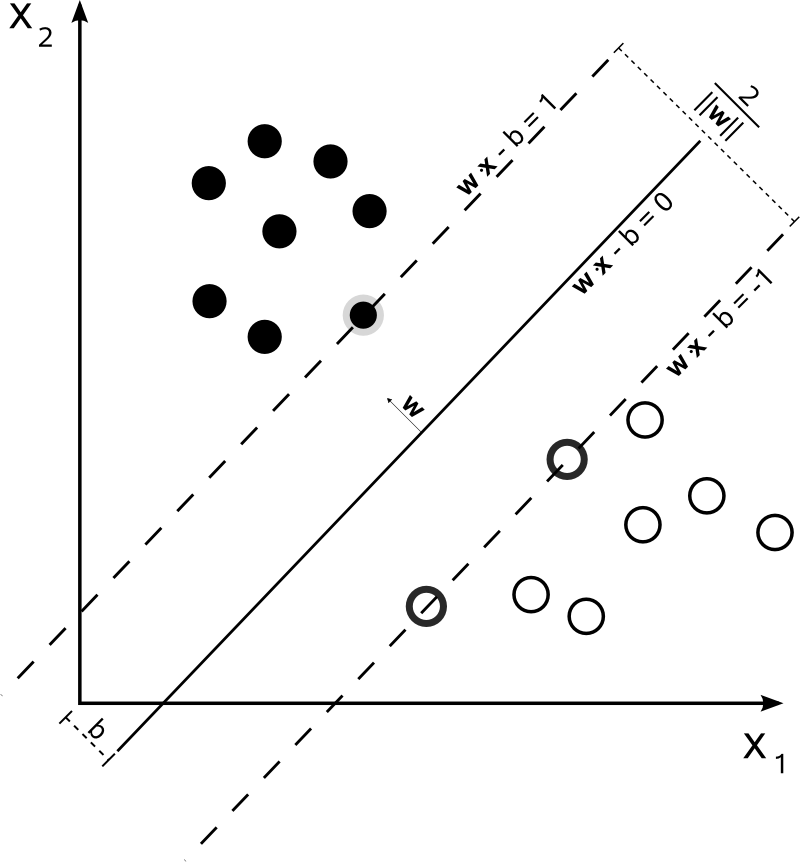
\includegraphics[width=0.4\textwidth]{figures/Svm_max_sep_hyperplane_with_margin}
\end{center}
\caption{{SVM} separating two class of points by a
         \emph{maximal margin hyperplane}. The hyperplane can be described by
         the collection of support vectors and associated weights, marked in the
         image as sample points with large borders.}
\label{fig:svm-sample}
\end{figure}

They have been used in several classification and recognition problems and are
in fact a standard across machine learning techniques. Their efficiency, exact
training results and generalization made them suitable for many tasks. Such as
text categorization, digit-recognition, spam-classification.
They have also been extensively used in visual place classification.
% TODO: add citations.

\subsection{Kernel-Trick}
\label{sec:kernel-trick}
Several classifiers can be modelled by requiring only the concept of inner\hyp{}product
between two samples. That product is often seen as a measure of distance or similarity
between the samples on some space. By using kernels it becomes possible to define such
space without explicit convert the samples to it. By abstracting the concept of distance
on such a kernel function it also becomes possible to use those classification methods
on strange data structures such as trees, strings or graphs.

For example \glspl{SVM}, in their basic form, are only able to handle linear spaces.
But the classes are most of the time not linearly separable in the input
space. Although there might exist a transformation $\phi$ from the original
space into a space $H$ where the input becomes linearly separable.

The Kernel trick allows to extend the \gls{SVM} definition to work on such space
$H$ without ever performing an implicit transformation between spaces. Being
enough for that to have a Kernel function defining an inner-product inside such
space: $K(x_i, x_j) = \phi(x_i)\cdot\phi(x_j)$.

Several kernel functions have been proposed being the most commonly used:

\begin{description}
\item[Polynomial Kernel] - $K(x, y) = (x \cdot y + p)^d$
\item[Radial Basis Function] - $K(x, y) = e^{-\gamma\|x - y \|^2}$
\item[Histogram Intersection] - $K(x, y) = e^{-\gamma \chi^2(x,y)}$, where
$\chi^2(x,y) = \sum_{i=1}^{N}\frac{(x_i-y_i)}{x_i+y_i}$ introduced by
\cite{barla2003histogram} allows to compute histogram similarity.
\item[Matching Kernels] - mimic matching similarity and are used when each
sample is represented as a set of features~\citep{boughorbel2005intermediate}.
\end{description}


\section{Features}
A feature is a piece of information which is expected to reveal information for
solving a specific task. Features are task-dependant and they will
yield different performance based on the type of task they are applied to.

A wanted property on features is its repeatability under similar conditions for
the problem in hand. This is: they should be stable and invariant across
unwanted types of transformations and noise. For example a visual feature for
object detection should be present even if the target object was translated,
scaled, rotated, the light-conditions have changed or even if the object is
partially occluded.

Extracting features with those properties allows to greatly reduce the size of
input by removing unwanted noise and useless information from the captured data.
Turning the classification problem easier, more reliable and more efficient.

Often several and different types of features need to be extracted. It has been
reported by \cite{pronobis2010ijrr} that using multiple features provides a
great benefit in the context of place classification.
And \cite{quattoni2009recognizing} has showed that different types have
different impact in indoor scene recognition based on the type of scene
matching. Specifically it was seen that some room-categories are more likely to be
recognized by the presence of some objects and others by it generic appearance.

In the context of robotics, sensors such as cameras, laser scans are used to
sense the surrounding environment, and features can be extracted from those.
Visual features can be seen as belonging to two categories:
\emph{local features} and \emph{global features}.


\subsection{Local Features}
\label{sec:local-features}
Local features describe fine grain properties of a part of image.
For example the existence of specific corner or an edge. \Gls{SIFT}
is an example of such feature and it been proven useful
for matching points between images and subsequence extension to object detection.

\subsubsection*{Interesting Points and SIFT}
\label{sec:sift}
The detection of interesting points has been studied for several years and is
the base of several computer vision problems solution. It allows to perform
point matching which can be used in several areas from image stitching,
3D reconstruction, video tracking, object detection, etc\dots

The most used method was presented by \cite{lowe1999object} and its based on
building a feature vector for each image. Each of those features is based on
\emph{interesting points} detected by the presence of maxima and minima of
difference of Gaussian functions applied in a scale-space.
The scale space is used to provide scale invariant detection. Gaussian functions
are used as they are the only way to model a linear scale-space.
Each interesting point is then described by a container that is rotation
invariant.

By seeing an object as a set of features points, index and matching is then
performed by a high-dimensional search on a database of know objects. After
matching objects can be verified for geometric coherence between features.
\Gls{SVM} classifiers can also be trained to detect objects based on this type
of local features by using \emph{Matching kernels} (\autoref{sec:kernel-trick}).

\begin{figure}[h]
    \centering
    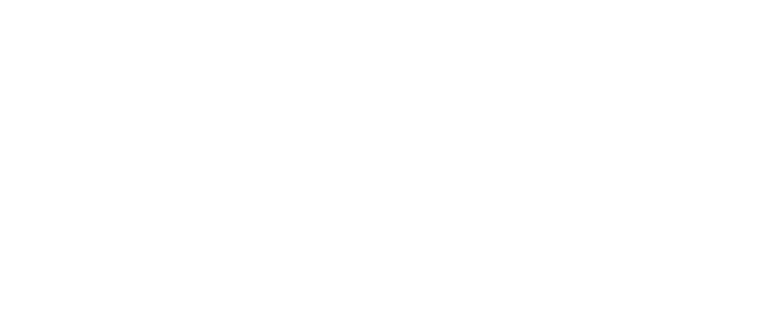
\includegraphics[width=0.8\textwidth]{figures/sift/sift.pdf}
    \caption{{SIFT} and other local features have been proven useful in object
             detection.}
\end{figure}


\subsection{Global Features}
Global features try to describe the whole image. E.g.\ either by
statistical analysis of features over all the image or by a structured
distribution of textures findable in the image.

\subsubsection*{Gist of a Scene}
\label{sec:gist}
Oliva and Torralba~\cite{oliva2006building} argue that fast scene recognition does not need to be
built on top of object recognition but can be analyzed by scene-centered
mechanisms.
They defend that position by pointing out behaviours on human vision:
when provided with a glance of a shot a person can identify the meaning of that
given shot or "gist of a scene" without remembering specific details.

As seen on \autoref{fig:gist} the gist is able to capture the dominant textural
features of the overall image and their coarse spatial layout~\citep{murphy2006object}.
With that, it is expected they serve the purpose of correctly describe the image
textures without the need to directly stored the original image.

\begin{figure}[h]
\center
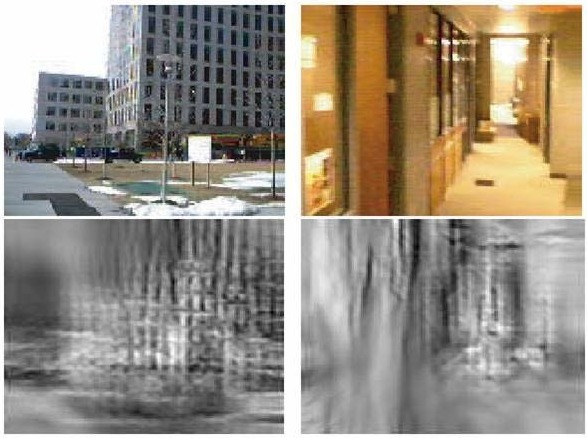
\includegraphics[width=0.60\textwidth]{figures/gist.jpg}
\caption{\label{fig:gist}An illustration of the gist of an image. Top row: original image I;
         bottom row: noise image J for which gist(I) = gist(J).}
\end{figure}


\subsubsection*{{CRFH} - Composed Receptive Field Histograms}
\label{sec:crfh}\label{sec:global-features}
\gls{CRFH} are a multidimensional statistical
representation of the occurrence of several image descriptors applied to an
image. They can be seen as an high-dimension histogram where each cell records
how many pixels of the image have the cell response for the applied descriptors.
Such high-dimensional histogram is expected to be able to describe global
information contained in the image by capturing several properties that co-occur
in a part of the image.
By using some techniques~\cite{linde2004object} several operations on those
high-dimensional histograms can be made computational efficient. This way not
only this descriptor discards part of the local information present on the image
but also allows to faster computations on similarity measures.


\begin{figure}[h]
\begin{center}
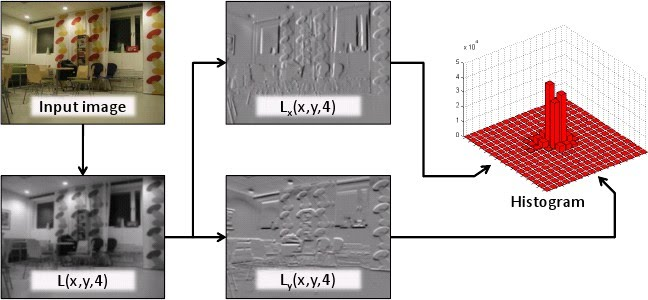
\includegraphics[width=1\textwidth]{figures/crfh_model.jpg}
\end{center}
\caption{A two dimensional histogram of the image built out from two image
         descriptors: $Lx$ and $Ly$. First-order Gaussian derivatives of image
         luminance in horizontal and vertical direction applied at a scale 4.}
\end{figure}

Multidimensional histograms have proven to be useful in the context of object
recognition~\citep{schiele1996object}. And have also been previously used in
the context of visual place classification~\cite{pronobis2010ijrr}.
\emph{Histogram intersection kernels} (\autoref{sec:kernel-trick}) can be used
to train classifiers based on this feature.


%%%%%%%%%%%%%%%%%%%%%%%%%%%%%%%%%%%%%%%%%%%%%%%%%%
% Important sections of this chapter begin here.
%%%%%%%%%%%%%%%%%%%%%%%%%%%%%%%%%%%%%%%%%%%%%%%%%%
\section{Probability Theory}
An important aspect when making decisions with noisy or missing information is
the uncertainty of the received information and of the final conclusion.
Probability theory comes to help by providing a framework able to deal with those
issues~\cite{bishop2006pattern}.

The key concept on it is that of \emph{probability}, which can be seen as way of
express the degree of belief that a certain event occurs.
When combined with decision theory it allows to perform optimal decisions with the
available information, even if it is ambiguous or incomplete.

A probability $P(x)$ of a given event $x$ is a value between $0$ and $1$, where $0$ means
the belief that $x$ will not occur and $1$ that it will certainly occur.
In cases $x$ does not specifies all the variables states that define the sample space, $P(x)$
is called a marginal probability. 

Often it is impossible to exactly describe the probability of a given event, in such cases
the concept of likelihood comes to help.
The likelihood of an event only has meaning when compared to one of another event.
In such case the ratio between both likelihoods will denote on how more likely an event is
over another.
When dealing with discrete and countable sample spaces any likelihood function can be converted
to a probability function by calculating the normalization factor such that the sum over all
the sample space is $1$.

\subsection{Conditional Probability}
It is also possible to denote the known information when calculating probabilities. For that
the notion of conditional probability is used $P(a|b)$. It denotes the probability of $a$
knowing that $b$ has occur. Often conditional probability is also represented by: $P_b(a)$.
In this thesis both notations will be used: the former for representing the information on
sensed variables and the second for representing information or assumptions on other generic
information such as graph structures.

Marginal probabilities can be related with conditional probabilities as described in the equation:
\begin{equation}
P(a|b) P(b)  = P(a, b)
\end{equation}


\section{Principle of Maximum Entropy}
\label{sec:max-entropy}
The principle of maximum entropy~\cite{shore1980axiomatic} states that when given
a set of distributions that are coherent with the acquired knowledge, the one which
maximizes entropy should be picked.

This can be used to select a distributions that most correctly describes the obtained
knowledge. For example, if all that is known from a distribution is the mean and deviation
then the correct approach is to model it with a normal distribution with the known parameters.
In case of having no information available, the uniform distribution shall be assumed.


\section{Probabilistic Graphical Models}
\label{sec:graphical-models}
% THIS IS ALL JUNK TEXT COPIED
Graphical models usage can be tracked back to earlies 1920 but they only become
popular in mid-eighties when researchers started to use \emph{Bayesian Networks}
to model expert systems~\citep{borgelt2002graphical}.

They serve as a better tool to model \emph{random variables}
(nodes on the graph) and their probabilities as they model the conditional
dependence between variables (edges on the graph). Important to note that here
\emph{random variables} does not denotes a truly random variable but one that is
unknown by the system and is conditioned by other variables/evidences.

This type of graphs provide a generative model where the probability of any
given scenario can be determined.
This means once a graphical model is learned, it can be used to generate new
samples from the learned distribution.

They have been successfully used in several machine-learning task such as:
information extraction, speech recognition, computer vision.
They are also useful due to their ability to deal with semantic (high-level)
features~\citep{boutell2006factor} and ability to represent properties of the
reality they try to model.

Two main types of graphical models are widely used: Bayesian Networks which model
directed edges between variables and Markov Random Fields where variables are
connected by a potential but no special direction is given to edges.

An important property of these graphs is the \emph{Markov-blanket} of a node.
For a given variable $a$, a \emph{Markov-blanket} is a set of variables in the
surroundings of $a$ that when given the value of $a$ becomes independent of the
rest of the graph~\citep{pearl1988probabilistic}.
On non-directional graphs it is directly determined by the nodes connected to $a$.
This allows the usage of graph algorithms such as \emph{min-cut} to quickly
determine most likely scenarios. In the case of directed edges a node blanket is
also influenced by the direction of the edges and more complex schemes need to
be used.

As \cite{lauritzen2002chain} points this two types of models can be represented
as a \emph{chain graph} where both directed and undirected edges can co-exist.
Though this generalization is hard to implement due to mis-understandings on the
concepts the graph-models use.

Another useful interpretation of graphical-models are \emph{factor graphs}.
Those are able to handle both \emph{Bayesian Networks} and
\emph{Markov Random Fields}. Under this interpretation a graph is seen as a
bipartite graph that connects variables with factors that influence
them~\citep{bishop2006pattern}.
This gives a very useful framework to develop belief propagation on them by
seeing a message-passing mechanism between nodes. Belief propagation is used to
calculate marginal-probabilities.

\begin{figure}[ht]
\centering

\subfloat[Bayes Networks] {
  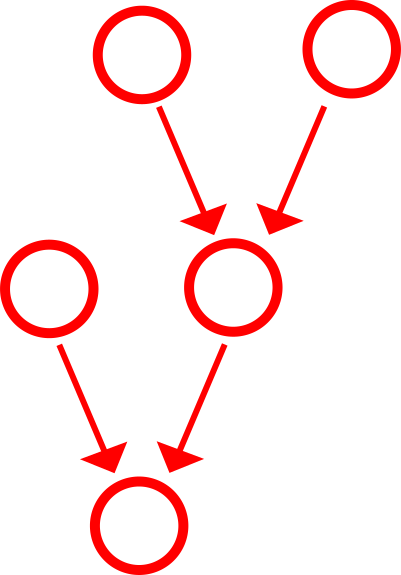
\includegraphics[width=0.2\textwidth]{figures/graphical-models/BayesNet.pdf}
}
\quad
\subfloat[Markov Random Field] {
  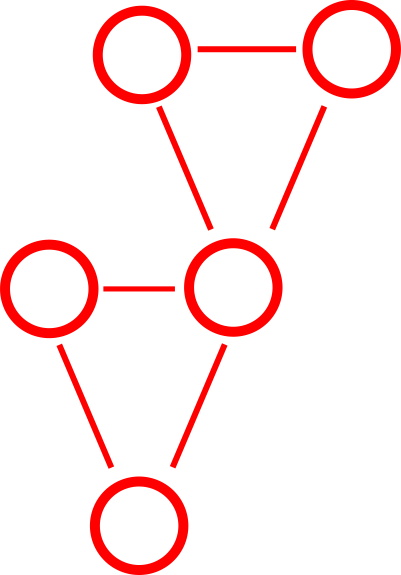
\includegraphics[width=0.2\textwidth]{figures/graphical-models/MarkovRandomField.pdf}
}
\quad
\subfloat[Factor Graph] {
  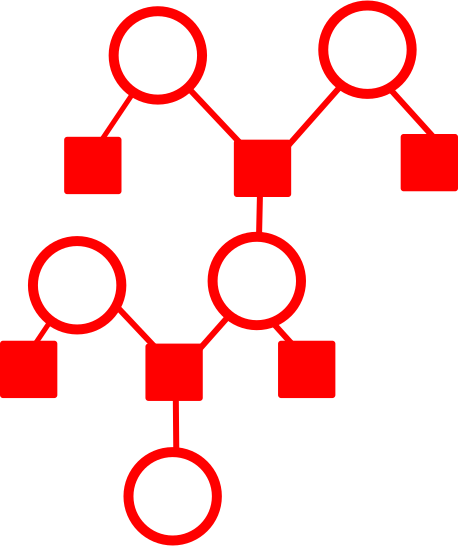
\includegraphics[width=0.3\textwidth]{figures/graphical-models/FactorGraph.pdf}
}
\end{figure}

\subsection{Factor Graphs}
A \emph{factor graph}~\cite{kschischang2001factor} is a bipartite graph connecting two sets of nodes $X_G$ and $F_G$
representing random variables and factors.
Each factor is described by function $\phi$ dependent only on the variables $x_\phi$
to which the factor is connected.
Thus, a factor graph can be seen as a description of probability density function obtained
by a product of all the factors. In order to represent the probability,
a normalization factor $Z$ needs to be introduced, resulting in the following equation:

\begin{equation}
P_G(x) = \frac{1}{Z}\prod_{\phi \in F_G}{\phi(x_{\phi})},\qquad
Z = \sum_{X_G}\prod_{\phi \in F_G}{\phi(x_{\phi})}
\end{equation}

\subsection{Inference}
The goal by obtaining a graphical model between all the variables of a system is the ability
to efficiently infer the most likely scenarios based on the available information.
The sensed information can be used to clamp variables and the model used to calculate probabilities
or marginal probabilities.

In that sense a basic operation on a graph is the \gls{MAP} operation, which allows to calculate
which configuration on a variable or subset of variables maximizes a given function.
